%%
%%
\documentclass[12pt]{book}
\usepackage{amsfonts}
\usepackage{amsmath}
\usepackage{amssymb}
\usepackage{graphicx}
\usepackage{hyperref}
\usepackage{float}
\usepackage{verbatim}

\usepackage{tasks}
%\NewTasks[style=enumerate,counter-format=tsk[A].,label-width=3ex]{choice}[\item](4)

\setlength{\textheight}{10in}
\setlength{\textwidth}{7.4in}
\setlength{\topmargin}{-0.75in}
\setlength{\oddsidemargin}{-0.5in}
\setlength{\evensidemargin}{-0.5in}
\setlength{\parskip}{0.15in}
\setlength{\parindent}{0in}



\begin{document}


\vspace{-1.0in}\begin{center}
\Large{MCV4UR : Advanced Placement Calculus and Vectors }

\Large{Assignment \#2}


\end{center}

%\medskip

\vspace{0.015in}\hrulefill\ 

\textbf{Reference Declaration} %  Fill in your Reference Declarations in this section before your submit your assignment.

Complete the Reference Declaration section below in order for your assigment to be graded.

If you used any references beyond the course text and lectures (such as other texts, discussions with colleagues or online resources), indicate this information in the space below.  If you did not use any aids, state this in the space provided. 

Be sure to cite appropriate theorems throughout your work. You may use shorthand for well-known theorems like the MVT, IVT, etc. 

Note: Your submitted work must be \textbf{your original work}. 

Family Name: Do\\%Family Name Here
First Name: Kien%First Name Here

Declared References:

Did some reading on how to find the tangent line given a point and the equation of a circle (hyperlinked):\\
- \href{https://doubleroot.in/lessons/circle/intersection-line-circle-1/}{Intersection of a Line and a Circle (Part 1)} \\
- \href{https://doubleroot.in/lessons/circle/tangent-slope-form-1/}{Tangent: Slope Form (Part 1)} 

Discussion with Phil Ostroscki on Question 7 about strategies and ways to tackle the problem.

% Type your references here.
% You can use as many lines as required.

\vspace{0.015in}\hrulefill\ 

\newpage

%%%%%%%%%%%% PROBLEMS START HERE

\begin{enumerate}

%% PROBLEM 1
\item Given $\cosh(x)=\dfrac{e^x + e^{-x}}{2}$, show the derivation of $\cosh^{-1}(x)$ as a function of $x$.\\

\textbf{Solution:}\\
First, let's represent $\cosh^{-1}(x)$ into something more familiar in order to find its derivative.\\
Let $y = \cosh^{-1}(x)$.
\begin{align}
    \cosh^{-1}(x) &= y \\
    \cosh(\cosh^{-1}(x)) &= \cosh(y) \\
    x &= \cosh(y) \\
    x &= \dfrac{e^y + e^{-y}}{2} \\
    2x &= e^y + \dfrac{1}{e^y} \\
    2xe^y&= (e^y)^2 + 1\\
    0 &= (e^y)^2 - 2x(e^y) + 1
\end{align}
Let $u = e^y$.
\begin{align}
    0 &= u^2 - 2xu + 1\\
    u &= \dfrac{2x\pm\sqrt{(2x)^2-4(1)(1)}}{2(1)} \\
    u &= \dfrac{2x\pm\sqrt{4x^2-4}}{2} \\
    u &= \dfrac{2x\pm\sqrt{4(x^2-1)}}{2} \\
    u &= \dfrac{2x\pm2\sqrt{x^2-1}}{2} \\
    u &= x\pm\sqrt{x^2-1} \\
    e^y &= x\pm\sqrt{x^2-1} \xleftarrow[]{\text{sub in }u \; = \; e^y} \\
    y &= \ln(x\pm\sqrt{x^2-1}) \\
    \cosh^{-1}(x) &= \ln(x\pm\sqrt{x^2-1}) \xleftarrow[]{\text{sub in }y \; = \; \cosh^{-1}(x)}
\end{align}
Now, we can determine $\dfrac{d}{dx}\cosh^{-1}(x)$. Let $y = \cosh^{-1}(x)$.
\begin{align}
    y &= \ln(x\pm\sqrt{x^2-1}) \\
    \dfrac{dy}{dx} &= \dfrac{1}{x \pm \sqrt{x^2-1}} \times \left(1 \pm \dfrac{d}{dx}\sqrt{x^2-1}\right) \xleftarrow[]{\text{by chain rule}} \\
    \dfrac{dy}{dx} &= \dfrac{1}{x \pm \sqrt{x^2-1}} \times \left(1 \pm \dfrac{1}{2\sqrt{x^2-1}} \times 2x\right) \xleftarrow[]{\text{by chain rule}} \\
    \dfrac{dy}{dx} &= \dfrac{1}{x \pm \sqrt{x^2-1}} \times \left(1 \pm \dfrac{x}{\sqrt{x^2-1}}\right) \\
    \dfrac{dy}{dx} &= \dfrac{1}{x \pm \sqrt{x^2-1}} \times \left( \dfrac{x \pm \sqrt{x^2-1}}{\sqrt{x^2-1}}\right) \\
    \dfrac{dy}{dx} &= \dfrac{1}{\sqrt{x^2-1}}
\end{align}


\newpage
\setcounter{equation}{0}
%% PROBLEM 2
\item Assume that $f(x)$ is continuous on the interval $J=[3,5]$, $f(3)=2$ and that $f'(x)=\dfrac{1}{1+x^3}$ on $J$. 

\begin{enumerate}
\item Determine the maximum and minimum values of $f'(x)$ on $J$. \\

\textbf{Solution:}\\
Let's take a look at $f'(x)$. I can see that as $x$ increases, $f'(x)$ decreases. That means $f'(x)$ is a decreasing function on $J$. Since 3 is the smallest value on $J$, I can say that $f'(3)$ is the largest value on $J$. Likewise, since 5 is the largest number on $J$, $f'(5)$ must be the smallest value on $J$.\\

\textbf{Therefore, the minimum and maximum value of $f'(x)$ on $J$ is $f'(5)$ and $f'(3)$, respectively.}\\

%%  2b
\item Prove that $\dfrac{127}{63} \le f(5) \le \dfrac{29}{14}$.\\

\textbf{Solution:}\\
Since $f'(x)$ has a max slope at $x=3$, a min slope at $x=5$, is positive on $J$ and decreases as $x$ increases, I can sketch out $f(x)$ starting with a steep slope then gradually getting less steep as $x$ increases. Note that the figure is not to scale.
\begin{figure}[H] %% figure 1
    \centering{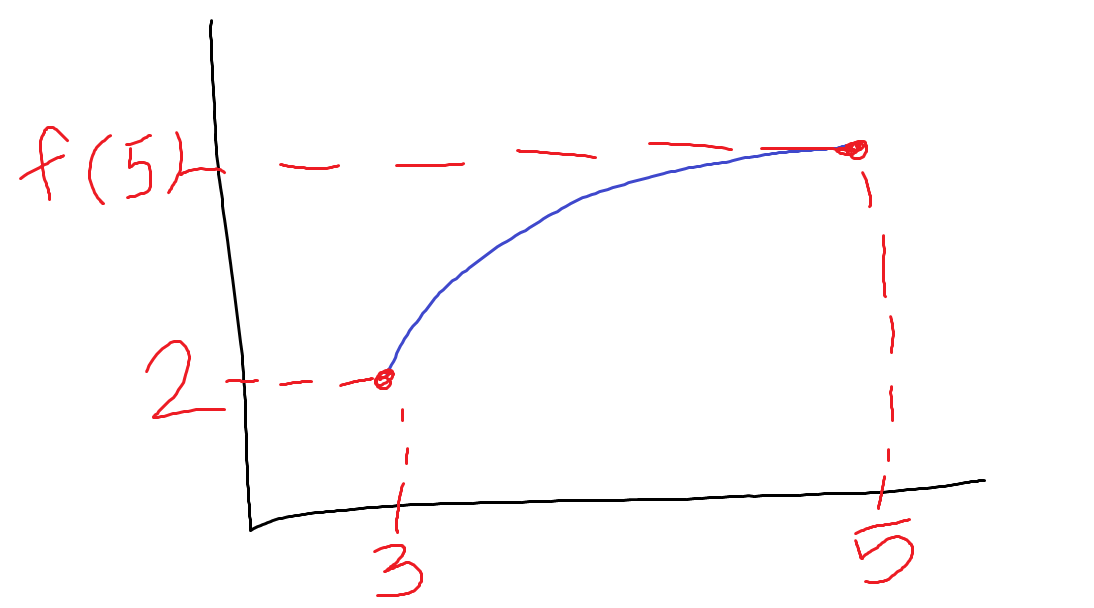
\includegraphics[width=6cm]{Q2bPhoto1.png}}
    \caption{Sketch of $f(x)$}
\end{figure} 
Determine the value of the maximum slope, $f'(3)$, and the minimum slope, $f'(5)$.
\begin{align}
    f'(3) &= \dfrac{1}{1+(3)^3} \\
    f'(3) &= \dfrac{1}{28} \\
    f'(5) &= \dfrac{1}{1+(5)^3} \\
    f'(5) &= \dfrac{1}{126}
\end{align}
\begin{figure}[H] %% figure 2
    \centering{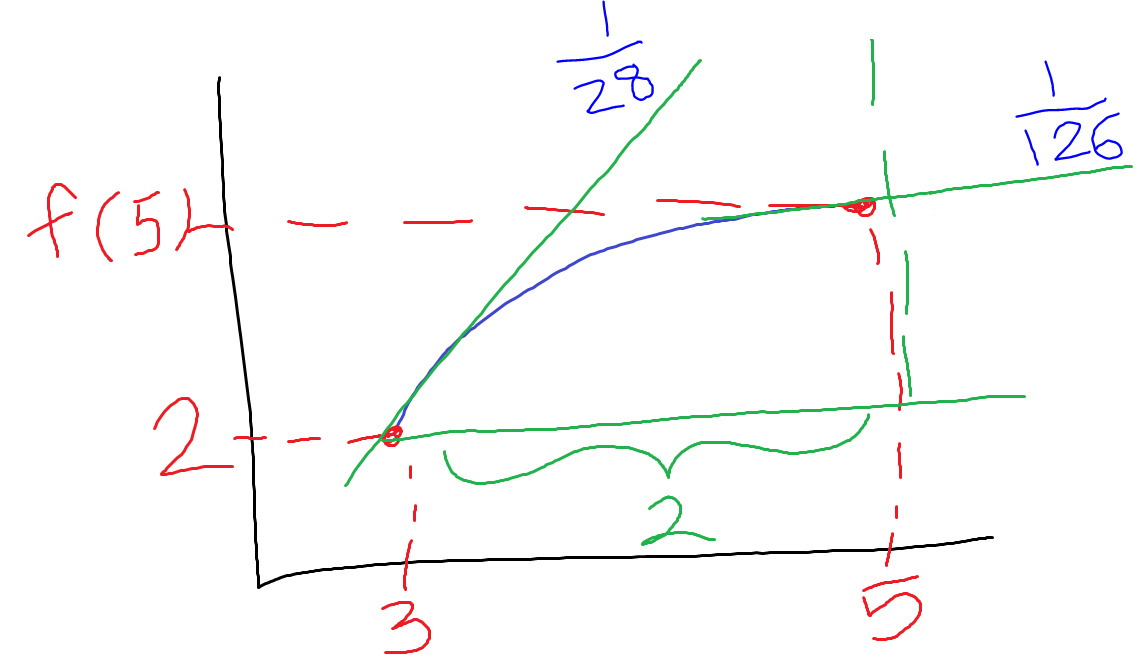
\includegraphics[width=6cm]{Q2bPhoto2.png}}
    \caption{Sketch of $f(x)$}
\end{figure}

We do not know $f(x)$ but now that we have determined the value of the max and min slopes of $f(x)$, we know that $\forall x \in J$, its minimum slope must be $\frac{1}{126}$ and its maximum slope must be $\frac{1}{28}$. So, let's assume the most extreme cases - that $f(x)$ is linear and that the entire function's slope is either the minimum or the maximum, ie: $f(x)$ has a slope of $\frac{1}{126}$ $\forall x \in J$ for case 1 and a slope of $\frac{1}{28}$ $\forall x \in J$ for case 2. With both of these extreme cases in mind, case 1 must yield the lowest possible outputs of $f(x)$ on $J$, similarly, case 2 must yield the highest possible outputs of $f(x)$ on $J$. See Figure 3.

\begin{comment}
Now that we have determined the value of the max and min slopes, we can assume that $f(x)$ on $[3,5]$ is linear and has a minimum slope of $\dfrac{1}{126}$ and a maximum slope of $\dfrac{1}{28}$. With this, we have two cases. The first case is that the slope of $f(x)$ on $J$ is $\dfrac{1}{126}$ which yields the lowest values of $f(x)$, and subsequently, the lowest value of $f(5)$. The second case is that the slope of $f(x)$ on $J$ is $\dfrac{1}{28}$ which yields the highest values of $f(x)$, and subsequently, the highest value of $f(5)$. See Figure 3.
\end{comment}

\begin{figure}[H] %% figure 3
    \centering{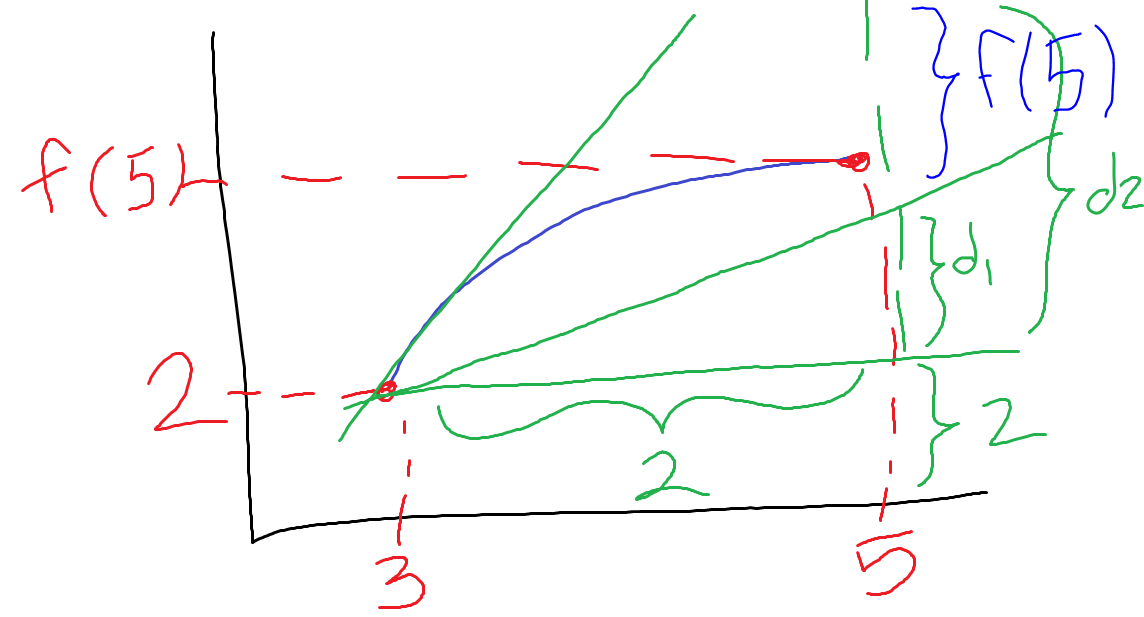
\includegraphics[width=6cm]{Q2bPhoto3.png}}
    \caption{Sketch of $f(x)$}
\end{figure}

We can see that all possible values for $f(5)$ is simply the difference between $2 + d_1$ and $2 + d_2$. First, let's determine $d_1$ and $d_2$.\\

Since a slope is the same as a tangent line and $\tan = \dfrac{opp.}{adj.}$, I can say, based on figure 2, that $\dfrac{1}{28} = \dfrac{d_1}{2}$. Likewise, I can say that $\dfrac{1}{126} = \dfrac{d_2}{2}$. For now, let's determine $d$ for both cases.\\
\begin{minipage}{0.5\textwidth}
    \begin{align*}
        \dfrac{1}{28} &= \dfrac{d_!}{2} \\
        d_1 &= \dfrac{1}{14}
    \end{align*}
\end{minipage}
\begin{minipage}{0.5\textwidth}
    \begin{align*}
        \dfrac{1}{126} &= \dfrac{d_2}{2} \\
        d_2 &= \dfrac{1}{63}
    \end{align*}
\end{minipage}\\

However, we are not done since we need to add 2 to $d_1$ and $d_2$ due to $f(3)$ starting at (3,2).
\begin{minipage}{0.5\textwidth}
    \begin{align*}
        f(5)_1 &= \dfrac{1}{14} + 2 \\
        f(5)_1 &= \dfrac{1}{14} + \dfrac{28}{14} \\
        f(5)_1 &= \dfrac{29}{14}
    \end{align*}
\end{minipage}
\begin{minipage}{0.5\textwidth}
    \begin{align*}
        f(5)_2 &= \dfrac{1}{63} + 2 \\
        f(5)_2 &= \dfrac{1}{63} + \dfrac{126}{63} \\
        f(5)_2 &= \dfrac{127}{63}
    \end{align*}
\end{minipage}\\

We cannot know the exact value of $f(5)$, however, we have just determined the maximum and minimum values for $f(5)$, therefore, $f(5)$ must be from $\dfrac{127}{63}$ to $\dfrac{29}{14}$, inclusive.\\

\textbf{Therefore, $\dfrac{127}{63} \leq f(5) \leq \dfrac{29}{14}$}.


\end{enumerate}

\newpage

%% PROBLEM 3
\item Consider a function $f(x)$.

\begin{enumerate}
\item Show that if $f(x)$ is differentiable on $\mathbb{R}$ and that $\forall x \in \mathbb{R} \, f'(x)=0$ , then $\forall x \in \mathbb{R} \, f(x)=f(0)$.\\

\textbf{Solution:}\\
Since $f(x)$ is differentiable on $\mathbb{R}$ and $f'(x) = 0$, or, the slope of $f(x)$ is 0 for all values of $x$, this means that that $f(x)$ is flat on the graph and $f(x) = C$ where $C$ is some constant (theorem 10.5 pg. 202). Since $f(x) = C$ for all values of $x$, $f(x) = f(0) = C$. \\

\item Assume that $f(x)$ is such that $\forall x \in \mathbb{R} \, f'(x)=f(x)$. Show that there exists a constant $C\in\mathbb{R}$ such that $f(x)=Ce^x$. 

(Hint: Let $g(x)=\dfrac{f(x)}{e^x}$ and show that it is a constant function.)\\

\textbf{Solution:}\\
Since $f'(x) = f(x)$ for all $x$, $f'(x) = f(x) = Ce^x$ or $f'(x) = f(x) = 0$.\\

For the first case, let $g(x) = \dfrac{f(x)}{e^x}$. Since $f(x) = Ce^x$ (in order to satisfy the given conditions), $g(x) = C$.\\

We will ignore the second case as it is not relevant to the question, and, that the answer is simply $g(x) = \dfrac{0}{e^x} = 0$.


\end{enumerate}


\newpage

%% PROBLEM 4
\item Given $f(x)=\dfrac{1}{x}$, prove $\forall n \in \mathbb{Z}^+$ that $f^{(n)}(x) = \dfrac{(-1)^n n!}{x^{n+1}}$. \\

\setcounter{equation}{0}
\textbf{Solution:}\\
By the Principle of Mathematical Induction, first we will check the to see if the Base Case is true, then we will come up with an Inductive Hypothesis, then we will use our Inductive Hypothesis to show that our statement holds.\\

\textbf{\underline{Base Case:}}\\
Show that the statement is true for the lowest value of $n$.\\
\begin{minipage}{0.5\textwidth}
    \begin{align*}
        f'(x) &= \dfrac{d}{dx} \left(\dfrac{1}{x}\right) \\
        f'(x) &= -\dfrac{1}{x^2}
    \end{align*}
\end{minipage}
\begin{minipage}{0.5\textwidth}
    \begin{align*}
        f'(x) &= \dfrac{(-1)^1 1!}{x^{1+1}} \\
        f'(x) &= \dfrac{-1}{x^2} \\
    \end{align*}
\end{minipage}
The base case is satisfied.\\

\textbf{\underline{Inductive Hypothesis:}}\\
Assume $f^{(k)}(x) = \dfrac{(-1)^k k!}{x^{k+1}}$ is true (n=k). We need to prove that $f^{(k+1)}(x) = \dfrac{(-1)^{k+1} (k+1)!}{x^{k+2}}$.\\

By definition, $f^{(k+1)}(x)$ is just the derivative of $f^{(k)}(x)$, so,  I just need to find the derivative of $f^{(k)} = \dfrac{(-1)^k k!}{x^{x+1}}$ and if it equals $f^{(k+1)}(x) = \dfrac{(-1)^{k+1} (k+1)!}{x^{k+2}}$, my hypothesis is correct.\\

\textbf{\underline{Proof:}}\\
Use the right side of $f^{(k)}(x) = \dfrac{(-1)^k k!}{x^{k+1}}$, determine $\dfrac{d}{dx} \left(\dfrac{(-1)^kk!}{x^{k+1}}\right)$. First of all, I can see that the\\\\ entire numerator is just a constant, so, let $z = (-1)^kk!$. We have,
\begingroup
\addtolength{\jot}{0.5em}
\begin{align}
    \dfrac{d}{dx} f^{(k)}(x) &= \dfrac{d}{dx} \left(\dfrac{z}{x^{k+1}}\right) \\
    \dfrac{d}{dx} f^{(k)}(x) &= \dfrac{z' (x^{k+1}) - z(x^{k+1})'}{ \left(x^{k+1}\right)^2 } \quad \xleftarrow[]{\text{quotient rule}} \\
    \dfrac{d}{dx} f^{(k)}(x) &= \dfrac{- z(k+1)x^{k}}{ x^{k+1} \times x^{k+1} } \\
    \dfrac{d}{dx} f^{(k)}(x) &= \dfrac{- z(k+1)}{ x \times x^{k+1} } \\
    \dfrac{d}{dx} f^{(k)}(x) &= \dfrac{- (-1)^k k!  (k+1)}{ x^{k+2} } \\
    \dfrac{d}{dx} f^{(k)}(x) &= \dfrac{(-1)^{k+1} (k+1)! }{ x^{k+2} } \\
    \dfrac{d}{dx} f^{(k)}(x) &= f^{(k+1)}(x)
\end{align}
\endgroup

\textbf{Therefore, $f^{(n)}(x) = \dfrac{(-1)^n n!}{x^{n+1}}$}



\newpage


%% PROBLEM 5
\item Hailstones originate at an altitude of about 3000 metres, although this varies. As they fall, air resistance slows down the hailstones considerably. In one model of air resistance, the speed (in metres per second) of a hailstone of mass $m$ as a function of time $t$ (in seconds) is given by $v(t) = \frac{mg}{k} (1 - e^{\frac{-kt}{m}})$ where $g \approx 9.8$ (in metres per second squared) is the acceleration due to gravity and $k$ is a constant that depends on the size of the hailstone and the conditions of the air. 

\begin{enumerate}
%% 5a
\item Determine the acceleration function $a(t)$ of the hailstone as a function of time.\\

\textbf{Solution:}\\
In order to $a(t)$, we simply have to find the derivative $v(t) = \dfrac{mg}{k}\left( 1 - e^{\frac{-kt}{m}} \right)$.
\setcounter{equation}{0}
\begingroup
\addtolength{\jot}{0.5em}
\begin{align}
    a(t) &= \dfrac{d}{dt} \left(\dfrac{mg}{k}\left( 1 - e^{\frac{-kt}{m}} \right) \right) \\
    a(t) &= \dfrac{d}{dt} \left( \dfrac{mg}{k} - \dfrac{mg}{k}e^{\frac{-kt}{m}} \right) \\
    a(t) &= - \dfrac{mg}{k} \left( \dfrac{-k}{m} \right)e^{\frac{-kt}{m}} \\
    a(t) &= g \times e^{\frac{-kt}{m}} \\
    a(t) &= 9.8 \times e^{\frac{-kt}{m}}
\end{align}
\endgroup



%% 5b
\item Determine $\lim\limits_{t\to \infty} v(t)$. What does this say about the speed of the hailstone?\\

\textbf{Solution:}
\setcounter{equation}{0}
\begingroup
\addtolength{\jot}{0.5em}
\begin{align}
    \lim\limits_{t\to \infty} v(t) &= \lim\limits_{t\to \infty} \left(\dfrac{mg}{k} (1 - e^{\frac{-kt}{m}}) \right) \\
    \lim\limits_{t\to \infty} v(t) &= \lim\limits_{t\to \infty} \left( \dfrac{mg}{k} - \dfrac{mg}{k}e^{\frac{-kt}{m}} \right)\\
    \lim\limits_{t\to \infty} v(t) &=  \dfrac{mg}{k} - \dfrac{mg}{k} \lim\limits_{t\to \infty} \left(e^{\frac{-kt}{m}} \right) \xleftarrow[\text{lim of constant times function = constant times lim of function}]{\text{lim of difference = difference of lim}} \\
    \lim\limits_{t\to \infty} v(t) &=  \dfrac{mg}{k} - \dfrac{mg}{k} \lim\limits_{t\to \infty} \left(\dfrac{1}{\sqrt[m]{e^{kt}}} \right) \\
    \lim\limits_{t\to \infty} v(t) &=  \dfrac{mg}{k} - \dfrac{mg}{k} \sqrt[m]{ \lim\limits_{t\to \infty} \left(\dfrac{1}{e^{kt}} \right)  } \\
    \lim\limits_{t\to \infty} v(t) &=  \dfrac{mg}{k} - \dfrac{mg}{k} \sqrt[m]{0  } \\
    \lim\limits_{t\to \infty} v(t) &=  \dfrac{mg}{k}
\end{align}
\endgroup

This means that as time approaches infinity, the velocity of the hailstone will be a constant,\\\\ $\dfrac{mg}{k}$, or, $\dfrac{9.8m}{k}$.

\newpage

%% 5c
\item Determine $\lim\limits_{t\to \infty} a(t)$. What does this say about the acceleration of the hailstone?\\

\textbf{Solution:}
\setcounter{equation}{0}
\begin{align}
    \lim\limits_{t\to \infty} a(t) &= \lim\limits_{t\to \infty} \left(9.8 \times e^{\frac{-kt}{m}}\right) \\
    \lim\limits_{t\to \infty} a(t) &= 9.8 \lim\limits_{t\to \infty} \dfrac{1}{\sqrt[m]{e^{kt}}} \\
    \lim\limits_{t\to \infty} a(t) &= 9.8 (0) \\
    \lim\limits_{t\to \infty} a(t) &= 0
\end{align}
This means that as time approaches infinity, there would be no acceleration on the hailstone.

\end{enumerate}

\newpage
\setcounter{equation}{0}
%% PROBLEM 6
\item Prove that if $\sqrt{x+y}-\sqrt{x-y}=1$ then $\frac{dy}{dx}$ can be expressed as a function of $y$.\\

\textbf{Solution:}\\
\begin{comment}
    %% ==================================
    \begingroup
    \addtolength{\jot}{0.7em}
    \begin{align}
        1 &= \sqrt{x+y} - \sqrt{x-y} \\
        \dfrac{dy}{dx} (1) &= \dfrac{d}{dx} \left(\sqrt{x+y} - \sqrt{x-y}\right) \\
        0 &= \dfrac{1}{2\sqrt{x+y}}\times\left(1+\dfrac{dy}{dx}\right) - \dfrac{1}{2\sqrt{x-y}}\times\left(1-\dfrac{dy}{dx}\right) \\
        0 &= \dfrac{1+y'}{2\sqrt{x+y}} - \dfrac{1-y'}{2\sqrt{x-y}} \\
        0 &= \dfrac{ (1+y')\sqrt{x-y} - (1-y')\sqrt{x+y} }{2\sqrt{x+y}\sqrt{x-y}} \\
        0 &= (1+y')\sqrt{x-y} - (1-y')\sqrt{x+y} \\
        0 &= \sqrt{x-y} + y'\sqrt{x-y} - \sqrt{x+y} + y'\sqrt{x+y} \\
        0 &= y' (\sqrt{x-y} + \sqrt{x+y}) + \sqrt{x-y} - \sqrt{x+y} \\
        y'&= \dfrac{\sqrt{x+y} - \sqrt{x-y}}{\sqrt{x-y} + \sqrt{x+y}} \\
        y'&= \dfrac{1}{\sqrt{x-y} + \sqrt{x+y}} \xleftarrow[]{\text{numerator = 1, given in the question}} \\
        y'&= \dfrac{1}{\sqrt{x-y} + \sqrt{x+y}} \times \dfrac{\sqrt{x+y} - \sqrt{x-y}}{\sqrt{x+y} - \sqrt{x-y}} \xleftarrow[\text{numerator = 1}]{\text{multiply by conjugate}} \\
        y'&= \dfrac{1}{x+y - x +y}\\
        y'&= \dfrac{1}{2y}\\
    \end{align}
    \endgroup
    %% ==================================
\end{comment}
\begingroup
\addtolength{\jot}{0.5em}
\begin{align}
    \sqrt{x+y} - \sqrt{x-y} &= 1\\
    \left(\sqrt{x+y} - \sqrt{x-y}\right)^2 &= 1^2\\
    x+y - 2\sqrt{x+y}\sqrt{x-y} +x-y &= 1 \xleftarrow[]{(a-b)^2\; =\; a^2-2ab+b^2}\\
    2x - 2 \sqrt{x+y}\sqrt{x-y} &= 1\\
    2(x -  \sqrt{x+y}\sqrt{x-y}) &= 1\\
    - \sqrt{x+y}\sqrt{x-y} &= \dfrac{1}{2} - x\\
    \left(- \sqrt{x+y}\sqrt{x-y}\right)^2 &= \left(\dfrac{1}{2} - x\right)^2\\
    (x+y)(x-y)  &= \dfrac{1}{4} - x + x^2 \xleftarrow[]{(a-b)^2\; =\; a^2-2ab+b^2}\\
    x^2 - xy + xy - y^2  &= x^2 -x + \dfrac{1}{4}\\
    -y^2 &= -x + \dfrac{1}{4} \\
    y^2 &= x - \dfrac{1}{4} \\
    \dfrac{d}{dx} \left(y^2\right) &= \dfrac{d}{dx} \left(x - \dfrac{1}{4}\right) \\
    2y \times \dfrac{dy}{dx} &= 1 \\
    \dfrac{dy}{dx} &= \dfrac{1}{2y}
\end{align}
\endgroup
\textbf{Therefore, $\dfrac{dy}{dx}$ can be expressed as a function of $y$.}



\newpage

\setcounter{equation}{0}
%% PROBLEM 7
\item Consider the three circles defined as $C_1 : x^2 + y^2 = 1$, $C_2 : (x-4)^2 + (y+1)^2 = 4$ and $C_3 : (x+5)^2 + (y-1)^2 = 9$. An \emph{external tangent} of two circles is a line that is tangent to both circles but does not pass between them. A pair of circles will have two external tangents.  

\begin{enumerate}
%%      7a =============================================
\item Determine the external tangents of $C_1$ and $C_2$.

%%      7b =============================================
\item Determine the external tangents of $C_1$ and $C_3$.

%%      7c =============================================
\item Determine the external tangents of $C_2$ and $C_3$.

%%      7d =============================================
\item Determine the points of intersection for each system of external tangents for each pair of circles.
%%      7e =============================================
\item Show that the points of intersection are collinear.
%%      7f =============================================
\item Conjecture, with evidence, whether you believe that the intersection points of these systems of external tangents for three circles will always be collinear or not. Cite any sources you use in your investigation.
\end{enumerate}
%% ================================================================
%%\newpage
\begin{comment} %% might be redundant
    Suppose we have a question where we are given an equation of a circle in the form $(x-a)^2 + (y-b)^2 = c^2$ where $a,b,c \in \mathbb{R}$ and a point on the graph $(x,y)$ that is not within the circle, and we are told to determine the two tangent lines to the circle from $(x, y)$. Determining the external tangent of two circles is simply an extension of this question in the sense that we are given the equations to two circles instead of one circle and a coordinate.
    
    So, we will determine the external tangents of $C_1$ and $C_2$, $C_1$ and $C_3$, as well as $C_2$ and $C_3$ using a similar method to determining the tangents to a circle from a coordinate.
\end{comment} %% ======== comment ============

\textbf{Solution for (a), (b) and (c):}

\textbf{Characteristics of a circle on a graph}\\
The general equation of a circle can be represented as $(x-a)^2+(y-b)^2 = c^2$ where $a,b,c \in \mathbb{R}$. In the equation of a circle, $a$ and $b$ translate the circle horizontally and vertically, respectively, and $c$ is the radius of the circle.

$(x+a)^2$ translates the circle left and $(x-a)^2$ translates the circle right.\\
\textit{Example:} $(x-2)^2 \xrightarrow{}$ trans. 2 units right.

Similarly, $(y+b)^2$ translates the circle down and $(y-b)^2$ translates the circle up.\\
\textit{Example:} $(y+3)^2 \xrightarrow{}$ trans. 3 units down.\\
\textit{Note:} These characteristics are important as we will refer to them later in the solution.

\textbf{Determine the general equation for the tangent slope for a circle}\\
Consider the circle $x^2+y^2=a^2$. At any point on the circumference of this circle, its tangent line must be in the form of a linear equation, $y=mx+c$. Determine the general equation for the tangent slope of the circle by subbing in $y=mx+c$ into $x^2+y^2=a^2$ and solve for $c$.
\begin{align}
    a^2 &= x^2 + y^2 \\
    a^2 &= x^2 + (mx+c)^2 \\
    a^2 &= x^2 + m^2x^2 + 2mcx + c^2 \\
    0 &= (1+m^2)x^2 + 2mcx + c^2 - a^2
\end{align}
The equation on line (4) is now in the quadratic form, $y=ax^2+bx+c$, where the coefficient of $x^2$ is $(1+m^2)$, the coefficient of $x$ is $2mc$ and the constant is $c^2-a^2$. Let's take a look at the discriminant of the quadratic formula ($\Delta = b^2-4ac$) and what it means. The discriminant, or, $\Delta$, can be one of three cases:

\textbf{Case 1:} $\Delta > 0\implies$  $y=mx+c$ runs through the circle and intersects two points on the circle's circumference.\\
\textbf{Case 2:} $\Delta < 0\implies$ $y=mx+c$ does not intersect the circle at all.\\
\textbf{Case 3:} $\Delta = 0\implies$ $y=mx+c$ only intersects the circle at one point.

Case 3 is also the tangent slope of a circle. Therefore, we will let $\Delta = 0$ and solve for $c$.\\

We have,
\begin{align}
    0 &= \Delta \\
    0 &= b^2 - 4ac \\
    0 &= (2mc)^2 - 4(1+m^2)(c^2-a^2) \\
    0 &= 4m^2c^2 - 4(c^2-a^2+m^2c^2-m^2a^2) \\
    0 &= m^2c^2 - (c^2-a^2+m^2c^2-m^2a^2) \\
    0 &= m^2c^2 - c^2+a^2-m^2c^2+m^2a^2 \\
    0 &=  - c^2+a^2+m^2a^2 \\
    c^2 &= a^2(1+m^2) \\
    c &= \pm a^2(1+m^2)
\end{align}
Now, subbing in $c$ from line (13) into $y=mx+c$, we have determined that the tangent of a circle can be represented as, $y = mx \pm a\sqrt{1+m^2}$ where $c$ is a constant, $a$ is radius of the circle, $m$ is the slope of the tangent equation.

\textbf{Connect the equation of a circle with the tangent of a circle}\\
Recall the equation of a circle can be represented as $(x-a)^2 + (y-b)^2 = c^2$ where $a,b,c \in \mathbb{R}$, $a,b$ translate the circle horizontally and vertically, respectively, and $c$ is the radius of the circle. We this equation of a circle to the tangent equation of a circle we determined earlier, but with the horizontal and vertical translations,
$$y = m(x-a) \pm c\sqrt{1+m^2} + b$$
where $a,b,c$ are the same as the equation of a circle (horizontal/vertical translation and radius) and $m$ is the slope of the tangent line. We can also see that we have two cases, $y = m(x-a) + c\sqrt{1+m^2} + b$ and $y = m(x-a) - c\sqrt{1+m^2} + b$.\\

\textbf{Determining the external tangents of $C_1$ and $C_2$}\\
$$C_1: \left(x\right)^{2}+\left(y\right)^{2}=1$$
$$C_2: \left(x-4\right)^{2}+\left(y+1\right)^{2}=4$$

First, we need to determine the $a, b, c$'s, or, the translations and the radii of $C_1, C_2$.\\
$C_1: a = 0, b = 0, c = 1$ \\
$C_2: a = -4, b = 1, c = 2$ \\

Now, we can write out their respective tangent equations by subbing values of $a,b,c$ into $$y = m(x-a) \pm c\sqrt{1+m^2} + b$$
we have,
$$C_{tan_1}: y = mx \pm 1\sqrt{1+m^2}$$ 
$$C_{tan_2}: y = mx-4m \pm 2\sqrt{1+m^2}-1$$
In order to determine the external tangents for $C_1$ and $C_2$, their respective tangents must be the same, therefore, let their tangents equal each other and determine the slope of the tangent, $m$.
\setcounter{equation}{0}
\begin{align}
    C_{tan_1} &= C_{tan_2} \\
    mx \pm 1\sqrt{1+m^2} &= mx-4m \pm \sqrt{1+m^2} - 1 \\
    \mp 2\sqrt{1+m^2} \pm \sqrt{1+m^2} &= mx-4m -mx - 1 \\
    \pm \sqrt{1+m^2} &= -4m - 1 \\
    \left(\pm \sqrt{1+m^2}\right)^2 &= (-4m - 1)^2 \\
    1+m^2 &= 16m^2 + 8m + 1\\
    0 &= 15m^2 + 8m
\end{align}
Now, I can determine $m$ using the quadratic formula.
\begin{align}
    m &= \dfrac{-b \pm \sqrt{b^2 -4ac}}{2a} \\
    m &= \dfrac{-8 \pm \sqrt{8^2 - 4(15)(0)}}{2(15)} \\
    m &= \dfrac{-8 \pm \sqrt{64}}{30} \\
    m &= \dfrac{-8 \pm 8}{30}
\end{align}

Therefore, $m_1 = 0$, $m_2 = \dfrac{-16}{30}$. \\

Now, we need to determine which slope goes with which pair of tangent lines. Recall that we have two cases,
$$mx + 1\sqrt{1+m^2} = mx-4m + 2\sqrt{1+m^2}-1 \qquad\qquad (1)$$
and
$$mx - 1\sqrt{1+m^2} = mx-4m - 2\sqrt{1+m^2}-1 \qquad\qquad (2)$$ 
In order to determine which slope goes with which pair, we can sub in $m_1$ into the first pair and if the left side equals the right side, $m_1$ belongs to the first pair, otherwise, it belongs to the second pair.\\

\textbf{Case 1:}\\
\begin{minipage}{0.5\textwidth}
    \begin{align*}
    &\textbf{LS}\\
        y &= (m_1)x + 1\sqrt{1+(m_1)^2} \\
        y &= (0)x + 1\sqrt{1+(0)^2} \\
        y &= 1\sqrt{1} \\
        y &= 1
    \end{align*}
\end{minipage}
\begin{minipage}{0.5\textwidth}
    \begin{align*}
    &\textbf{RS}\\
        y &= (m_1)x-4(m_1) + 2\sqrt{1+(m_1)^2}-1 \\
        y &= 0(x-4) + 2\sqrt{1+0^2} - 1\\
        y &= 2\sqrt{1} - 1\\
        y &= 1
    \end{align*}
\end{minipage}\\

The left side equals the right side, therefore, $m_1$ goes with the first external tangent equation and $m_2$ goes with the second external tangent equation. With this, we also have our first external tangent, $y=1$.

\newpage

Now I can determine the second external tangent using either side of the second external tangent equation, but just to be cautious, I will use both sides of the equation similar to how I determined the external tangent for the first equation.\\

\textbf{Case 2:}\\
\begingroup
\addtolength{\jot}{0.8em}
\begin{minipage}{0.5\textwidth}
    \begin{align*}
    &\textbf{LS}\\
        y &= (m_2)x - 1\sqrt{1+(m_2)^2} \\
        y &= \left(\dfrac{-16}{30}\right)x - 1\sqrt{1+\left(\dfrac{-16}{30}\right)^2} \\
        y &= \dfrac{-16}{30}x - \dfrac{17}{15}
    \end{align*}
\end{minipage}
\endgroup
\begingroup
\addtolength{\jot}{0.3em}
\begin{minipage}{0.5\textwidth}
    \begin{align*}
    &\textbf{RS}\\
        y &= (m_2)x-4(m_2) - 2\sqrt{1+(m_2)^2}-1 \\
        y &= \left(\dfrac{-16}{30}\right)x-4\left(\dfrac{-16}{30}\right) - 2\sqrt{1+\left(\dfrac{-16}{30}\right)^2}-1 \\
        y &= \dfrac{-16}{30}x + \dfrac{32}{15} - \dfrac{34}{15} - 1\\
        y &= \dfrac{-16}{30}x - \dfrac{17}{15}
    \end{align*}
\end{minipage}
\endgroup

Therefore, our second tangent is $y = \dfrac{-16}{30}x - \dfrac{17}{15}$.

$\therefore$ \textbf{The external tangents of $C_1$ and $C_2$ are } $y = 1$ \textbf{and} $y=\dfrac{-16}{30}x - \dfrac{17}{15}$.\\

With the same method, I can determine the external tangents of $C_2$, $C_3$ and $C_1$, $C_3$.\\

%% ============================================================

\textbf{Determining the external tangents of $C_1$ and $C_3$}\\
First, we write the equations of the circles,
$$C_1: \left(x\right)^{2}+\left(y\right)^{2}=1$$
$$C_3: \left(x+5\right)^{2}+\left(y-1\right)^{2}=9$$
then, we sub in their translations and radii into the linear tangent equation $y = m(x-a) \pm c\sqrt{1+m^2} + b$ so that we have,
$$C_{tan_1}: y=mx \pm \sqrt{1+m^{2}}$$
$$C_{tan_3}: y=mx + 5m \pm 3\sqrt{1+m^{2}}+1$$
Now, let $C_{tan_1} = C_{tan_3}$, rewrite the equation into quadratic equation, then determine the slope, $m$.
\begin{align}
    C_{tan_1} &= C_{tan_3} \\
    mx \pm \sqrt{1+m^{2}} &= mx + 5m \pm 3\sqrt{1+m^{2}}+1 \\
    \pm \sqrt{1+m^{2}} \mp 3\sqrt{1+m^{2}} &= mx - mx + 5m + 1 \\
    \pm2\sqrt{1+m^{2}} &= 5m + 1 \\
    \left(\pm2\sqrt{1+m^{2}}\right)^2 &= (5m + 1)^2 \\
    4(1+m^2) &= (5m)^2 + 2(5m)(1) + 1^2 \\
    4+4m^2 &= 25m^2 + 10m + 1 \\
    0 &= 21m^2 + 10m - 3
\end{align}
Determine $m$ using the quadratic formula.
\begin{align}
    &= \dfrac{-10 \pm \sqrt{10^2 - 4(21)(-3)}}{2(21)} \\
    &= \dfrac{-5\pm2\sqrt{22}}{21}
\end{align}
Therefore, $m_1 = \dfrac{-5-2\sqrt{22}}{21}$ and $m_2 = \dfrac{-5+2\sqrt{22}}{21}$.\\

Determine which slope goes with which case by subbing the slope into each case,
$$mx + \sqrt{1+m^{2}} = mx + 5m + 3\sqrt{1+m^{2}}+1 \qquad \qquad (1)$$
$$mx - \sqrt{1+m^{2}} = mx + 5m - 3\sqrt{1+m^{2}}+1 \qquad \qquad (2)$$
\textbf{Case 1: LS}
\begin{align}
    y &= (m_1)x + \sqrt{1+(m_1)^{2}} \\
    y &= \left(\dfrac{-5-2\sqrt{22}}{21}\right)x + \sqrt{1+ \left(\dfrac{-5-2\sqrt{22}}{21}\right)^2}
\end{align}
\textbf{Case 1: RS}
\begin{align}
    y &= (m_1)x + 5(m_1) + 3\sqrt{1+(m_1)^{2}}+1 \\
    y &=  \left(\dfrac{-5-2\sqrt{22}}{21}\right)(x)+5\left(\dfrac{-5-2\sqrt{22}}{21}\right)+3\sqrt{1+ \left(\dfrac{-5-2\sqrt{22}}{21}\right)^2}+1 \\
    y &= \left(\frac{-5-2\sqrt{22}}{21}\right)x+\sqrt{1+\left(\frac{-5-2\sqrt{22}}{21}\right)^{2}}
\end{align}
Therefore, the first external tangent of $C_1$ and $C_3$ is $y=\left(\frac{-5-2\sqrt{22}}{21}\right)x+\sqrt{1+\left(\frac{-5-2\sqrt{22}}{21}\right)^{2}}$

\textbf{Case 2: LS}
\begin{align}
    y &= (m_2)x - \sqrt{1+(m_2)^{2}} \\
    y &= \left(\dfrac{-5+2\sqrt{22}}{21}\right)x - \sqrt{1+ \left(\dfrac{-5+2\sqrt{22}}{21}\right)^2}
\end{align}
\textbf{Case 2: RS}
\begin{align}
    y &= (m_2)x + 5(m_2) - 3\sqrt{1+(m_2)^{2}}+1 \\
    y &=  \left(\dfrac{-5+2\sqrt{22}}{21}\right)(x)+5\left(\dfrac{-5+2\sqrt{22}}{21}\right)-3\sqrt{1+ \left(\dfrac{-5+2\sqrt{22}}{21}\right)^2}+1 \\
    y &= \left(\frac{-5+2\sqrt{22}}{21}\right)x-\sqrt{1+\left(\frac{-5+2\sqrt{22}}{21}\right)^{2}}
\end{align}
Therefore, the second external tangent of $C_1$ and $C_3$  is $y=\left(\frac{-5+2\sqrt{22}}{21}\right)x-\sqrt{1+\left(\frac{-5+2\sqrt{22}}{21}\right)^{2}}$\\

$\therefore$ \textbf{The external tangents of $C_1$ and $C_3$ are } $$y=\left(\frac{-5-2\sqrt{22}}{21}\right)x+\sqrt{1+\left(\frac{-5-2\sqrt{22}}{21}\right)^{2}}$$  \textbf{and} $$y=\left(\frac{-5+2\sqrt{22}}{21}\right)x-\sqrt{1+\left(\frac{-5+2\sqrt{22}}{21}\right)^{2}}$$\\

%% ===================================================

\textbf{Determining the external tangents of $C_2$ and $C_3$}\\
The equations of the circles,
$$C_2: \left(x-4\right)^{2}+\left(y+1\right)^{2}=4$$
$$C_3: \left(x+5\right)^{2}+\left(y-1\right)^{2}=9$$
then, we sub in their translations and radii into the linear tangent equation $y = m(x-a) \pm c\sqrt{1+m^2} + b$ so that we have,
$$C_{tan_2}: y=m\left(x-4\right)-2\sqrt{1+m^{2}}-1$$
$$C_{tan_3}: y=m\left(x+5\right)-3\sqrt{1+m^{2}}+1$$
or,
$$C_{tan_2}: y=mx - 4m \pm 2\sqrt{1+m^{2}} - 1$$
$$C_{tan_3}: y=mx + 5m \pm 3\sqrt{1+m^{2}} + 1$$
Now, let $C_{tan_2} = C_{tan_3}$, rewrite the equation into quadratic equation, then determine the slope, $m$.
\begin{align}
    C_{tan_2} &= C_{tan_3} \\
    mx - 4m \pm 2\sqrt{1+m^{2}} - 1 &= mx + 5m \pm 3\sqrt{1+m^{2}}+1 \\
    \pm\sqrt{1+m^{2}} &= 9m +2\\
    \left(\pm\sqrt{1+m^{2}}\right)^2 &= (9m +2)^2 \\
    1+m^2 &= (9m)^2 + 2(9m)(2) + 2^2 \\
    0 &= 81m^2 + 36m + 4 -m^2-1 \\
    0 &= 80m^2 + 36m + 3
\end{align}
Determine $m$ using the quadratic formula.
\begin{align}
    &= \dfrac{-36 \pm \sqrt{36^2 - 4(80)(3)}}{2(80)} \\
    &= \dfrac{-9\pm \sqrt{21}}{40}
\end{align}
Therefore, $m_1 = \dfrac{-9- \sqrt{21}}{40}$ and $m_2 = \dfrac{-9+ \sqrt{21}}{40}$.\\

Determine which slope goes with which case by subbing the slope into each case,
$$mx - 4m + 2\sqrt{1+m^{2}} - 1 = mx + 5m + 3\sqrt{1+m^{2}}+1 \qquad \qquad (1)$$
$$mx - 4m - 2\sqrt{1+m^{2}} - 1 = mx + 5m - 3\sqrt{1+m^{2}}+1 \qquad \qquad (2)$$
\textbf{Case 1: LS}
\begin{align}
    y &= (m_1)x - 4(m_1) + 2\sqrt{1+(m_1)^{2}} - 1 \\
    y &= \left(\dfrac{-9- \sqrt{21}}{40}\right)x - 4\left(\dfrac{-9- \sqrt{21}}{40}\right) +2\sqrt{1+\left(\dfrac{-9- \sqrt{21}}{40}\right)^2} -1 \\
    y &= \left(\dfrac{-9- \sqrt{21}}{40}\right)x + 2.470416
\end{align}
\textbf{Case 1: RS}
\begin{align}
    y &= (m_1)x + 5(m_1) + 3\sqrt{1+(m_1)^{2}}+1 \\
    y &=  \left(\dfrac{-9- \sqrt{21}}{40}\right)(x)+5\left(\dfrac{-9- \sqrt{21}}{40}\right)+3\sqrt{1+ \left(\dfrac{-9- \sqrt{21}}{40}\right)^2}+1 \\
    y &= \left(\dfrac{-9- \sqrt{21}}{40}\right)x + 2.470416
\end{align}
Therefore, the first external tangent of $C_2$ and $C_3$ is $y = \left(\dfrac{-9- \sqrt{21}}{40}\right)x + 2.470416$

\textbf{Case 2: LS}
\begin{align}
    y &= (m_2)x - 4(m_2) - 2\sqrt{1+(m_2)^{2}} - 1 \\
    y &= \left(\dfrac{-9+ \sqrt{21}}{40}\right)x - 4\left(\dfrac{-9+ \sqrt{21}}{40}\right) - 2\sqrt{1+\left(\dfrac{-9+ \sqrt{21}}{40}\right)^{2}} - 1 \\
    y &= \left(\dfrac{-9+ \sqrt{21}}{40}\right)x - 2.570416
\end{align}
\textbf{Case 2: RS}
\begin{align}
    y &= (m_2)x + 5(m_2) - 3\sqrt{1+(m_2)^{2}}+1 \\
    y &= \left(\dfrac{-9+ \sqrt{21}}{40}\right)(x)+5\left(\dfrac{-9+ \sqrt{21}}{40}\right)-3\sqrt{1+ \left(\dfrac{-9+ \sqrt{21}}{40}\right)^2}+1 \\
    y &= \left(\dfrac{-9+ \sqrt{21}}{40}\right)x - 2.570416
\end{align}
Therefore, the second external tangent of $C_2$ and $C_3$  is $y = \left(\dfrac{-9+ \sqrt{21}}{40}\right)x - 2.570416$\\

$\therefore$ \textbf{The external tangents of $C_2$ and $C_3$ are } $$y=\left(\dfrac{-9- \sqrt{21}}{40}\right)x + 2.470416$$  \textbf{and} $$y=\left(\dfrac{-9+ \sqrt{21}}{40}\right)x - 2.570416$$\\
%% ===================================================
\setcounter{equation}{0}
\textbf{Solution for (d):}\\
Since each system of external tangents has two linear equations, I can simply determine the points of intersection by elimination or substitution.\\

%% ===================================================

\textbf{Point of intersection of the $C_1$ and $C_2$'s external tangents}\\
Tangent equation 1: $$y=1$$
Tangent equation 2: $$y=\dfrac{-16}{30}x-\dfrac{17}{15}$$
Determine the point of intersection by substitution.
\begingroup
\addtolength{\jot}{0.5em}
\begin{align}
    1 &= \dfrac{-16}{30}x-\dfrac{17}{15}\\
    x &= \dfrac{32}{15} \times \dfrac{30}{-16} \\
    x &= -4
\end{align}
\endgroup
We already know $y=1$, \\

$\therefore$ $C_1$ and $C_2$'s tangent lines have a point of intersection at $(-4,1)$. \\

%% ===================================================

\textbf{Point of intersection of the $C_1$ and $C_3$'s external tangents}\\
Tangent equation 1: $$y=\left(\frac{-5-2\sqrt{22}}{21}\right)x+\sqrt{1+\left(\frac{-5-2\sqrt{22}}{21}\right)^{2}}$$
Tangent equation 2: $$y=\left(\frac{-5+2\sqrt{22}}{21}\right)x-\sqrt{1+\left(\frac{-5+2\sqrt{22}}{21}\right)^{2}}$$
Determine the point of intersection by substitution.
\begingroup
\addtolength{\jot}{0.5em}
\begin{align}
    \left(\frac{-5-2\sqrt{22}}{21}\right)x+\sqrt{1+\left(\frac{-5-2\sqrt{22}}{21}\right)^{2}} &= \left(\frac{-5+2\sqrt{22}}{21}\right)x-\sqrt{1+\left(\frac{-5+2\sqrt{22}}{21}\right)^{2}} \\
    x &= 2.5
\end{align}
\endgroup
Sub $x=2.5$ into tangent equation 1 to determine the $y$ coordinate.
\begin{align}
    y &= \left(\frac{-5-2\sqrt{22}}{21}\right)x+\sqrt{1+\left(\frac{-5-2\sqrt{22}}{21}\right)^{2}} \\
    y &= \left(\frac{-5-2\sqrt{22}}{21}\right)(2.5)+\sqrt{1+\left(\frac{-5-2\sqrt{22}}{21}\right)^{2}}\\
    y &= -0.5
\end{align}

$\therefore$ $C_1$ and $C_3$'s tangent lines have a point of intersection at $(2.5,-0.5)$. \\

%% ===================================================

\textbf{Point of intersection of the $C_2$ and $C_3$'s external tangents}\\
Tangent equation 1: $$y=\left(\dfrac{-9- \sqrt{21}}{40}\right)x + 2.470416$$
Tangent equation 2: $$y=\left(\dfrac{-9+ \sqrt{21}}{40}\right)x - 2.570416$$
Determine the point of intersection by substitution.
\begingroup
\addtolength{\jot}{0.5em}
\begin{align}
    \left(\dfrac{-9- \sqrt{21}}{40}\right)x + 2.470416 &= \left(\dfrac{-9+ \sqrt{21}}{40}\right)x - 2.570416 \\
    x &= 22
\end{align}
\endgroup
Sub $x=22$ into tangent equation 1 to determine the $y$ coordinate.
\begin{align}
    y &= \left(\dfrac{-9- \sqrt{21}}{40}\right)x + 2.470416 \\
    y &= \left(\dfrac{-9- \sqrt{21}}{40}\right)(22) + 2.470416 \\
    y &= -5
\end{align}

$\therefore$ $C_2$ and $C_3$'s tangent lines have a point of intersection at $(22,-5)$. \\

\textbf{Solution for (f):}\\
Suppose we have three circles defined as $S_1: x^2 + y^2 = 4$, $S_2: \left(x-6\right)^{2}+\left(y\right)^{2}=4$ and $S_3: \left(x-3\right)^{2}+\left(y+6\right)^{2}=4$. Since all of their radii are the same, the external tangents in each system must be parallel. If each system only has parallel tangents, there are no points of intersection. If there are no points of intersection, the "points of intersection" cannot be collinear.





\end{enumerate}
\end{document} 
